\chapter{Numerical Results}
\label{sec:results}

\cleanchapterquote{In the end, a theory is accepted not because it is confirmed by conventional empirical tests, but because researchers persuade one another that the theory is correct and relevant.}{Fisher Black}{(1938-1995)}

Having calibrated our models, now we are able to price the FX-TARN with the different methods we have studied. This chapter presents the results of experiments on simplified FX-TARN, described in Section \ref{sec:res:setup}. Then, in Section \ref{sec:res:results}, we will expose all the results in the three different cases of redemption, i.e. No gain, Part gain and Full gain. Next, in Section \ref{sec:res:analysis}, we will study the speed, the accuracy and the convergence of the Finite Difference and Convolution methods. Finally, to conclude this chapter with Section \ref{sec:res:TS}, we will price the term sheet example that we have introduced in the introduction.

\section{Experimental setup}
\label{sec:res:setup}
The programming was done in \textsc{Matlab} and run on a MacBook Pro with 2 GHz Intel Core i5 processor and 8 Go RAM. To be more accurate in the analysis of the results and don't waste time in computation, we have chosen to price a simplified FX-TARN. 

Consider the same FX-TARN as in our term sheet example with only 6 fixing dates over one year and constant strike $K = 0.942$ and accrual amount per fixing date $N_f=1$. Recall the underlying foreign exchange rate is the USD/CHF on 23 May 2017 with $S_0 = 0.9730$. The deposit rates of USD and CHF are respectively given by $r_f = 1.197\%$ and $r_d = -1.237\%$ at 1Y maturity. Finally, the target level is settled at $0.4$. We will treat the three different types of knock-out condition, i.e. No gain, Part gain and Full gain.

The error of the methods will be presented as the absolute value of the difference between the calculated value and a reference value, $|V(S_0,t_0,0)-V_\text{ref}(S_0,t_0,0)|$. We choose the reference value to be the value computed with a very thin discretization in convolution method, i.e. $N_x = 2\cdot10^4,N_a = 2\cdot10^3$. This choice is motivated by the fact that the other methods are too expensive in computational cost for a similar accuracy. In particular, the computations of prices under jump-diffusion models in Monte Carlo are very slow since we have to simulate a lot of random variables that modeled the jumps in addition to the diffusion path. However, we can compare the results of $10^8$ simulations versus the reference values under Black-Scholes, NIG and VG models, (cf. Tables \ref{tab:ref_ng}, \ref{tab:ref_pg} and \ref{tab:ref_pg}).

\begin{table}[!ht]
\centering
  \begin{tabular}{l||c|c|c}
    \toprule
    No gain & $V_\text{ref}$ & $V_\text{MC}$ & SE \\
    \toprule
   Black-Scholes & $0.15877$ & $0.15876$ & $1.33\cdot10^{-5}$\\
   NIG 			 & $0.16166$ & $0.16165$ & $1.28\cdot10^{-5}$\\
   VG 			 & $0.16246$ & $0.16248$ & $1.29\cdot10^{-5}$\\
    \bottomrule
  \end{tabular}
  \vspace{5pt}
  \caption{\label{tab:ref_ng} No gain TARN reference value in comparison with $10^7$ Monte Carlo simulations.}
\end{table}

\begin{table}[!ht]
\centering
  \begin{tabular}{l||c|c|c}
    \toprule
    Part gain & $V_\text{ref}$ & $V_\text{MC}$ & SE \\
    \toprule
   Black-Scholes 	& $0.16863$ & $0.16861$ & $1.46\cdot10^{-5}$\\
   NIG 				& $0.17093$ & $0.17094$ & $1.41\cdot10^{-5}$\\
   VG 				& $0.17181$ & $0.17180$ & $1.42\cdot10^{-5}$\\
    \bottomrule
  \end{tabular}
  \vspace{5pt}
  \caption{\label{tab:ref_pg} Part gain TARN reference value in comparison with $10^7$ Monte Carlo simulations.}
\end{table}

\begin{table}[!ht]
\centering
  \begin{tabular}{l||c|c|c}
    \toprule
    Full gain & $V_\text{ref}$ & $V_\text{MC}$ & SE \\
    \toprule
   Black-Scholes 	& $0.17763$ & $0.17763$ & $1.62\cdot10^{-5}$\\
   NIG 				& $0.17929$ & $0.17927$ & $1.57\cdot10^{-5}$\\
   VG 				& $0.18024$ & $0.18026$ & $1.57\cdot10^{-5}$\\
    \bottomrule
  \end{tabular}
  \vspace{5pt}
  \caption{\label{tab:ref_fg} Full gain TARN reference value in comparison with $10^7$ Monte Carlo simulations.}
\end{table}

We can see that the reference value is very closed to the Monte Carlo value and the standard error of $1.28\cdot 10^{-5}$ to $1.62\cdot 10^{-5}$ confirm that our choice is not so bad. Then, we can hope that the reference value for the Merton and Kou models are closed to the true value.

\section{Results}
\label{sec:res:results}
In this section, we just define the settings of the experiments and expose the numerical results. We will discuss the results properties in the following section.
\subsection{Settings}
Concerning the Finite difference method, we fixed 
\begin{align*}
x_{\min} &= -5, \qquad x_{\max} = 1,\\
q_{\min} &= x_{\min}-B_l = -7, \\
q_{\max} &= x_{\max}+B_r = 3, \\
\epsilon &= 0.05.
\end{align*}
$x_{\min}$ and $x_{\max}$ were chosen such that $S_{\min} = e^{x_{\min}}$ and $S_{\max}=e^{x_{\max}}$ are far from $S_0$. Then $q_{\min}$ and $q_{\max}$ were chosen such that the L\'evy density centered in $x_{\min}$ and $x_{\max}$ is closed to zero on $q_{\min}$ and $q_{\max}$ as we can see in figure \ref{fig:qmin-qmax}. This is necessary to treat correctly the integral term in the PIDE. The choice of the parameter $\epsilon$ was a bit more complicated since the error of the method is given by
$$error \sim \epsilon + C(\epsilon) \Delta x^2 + \Delta t,$$
and $C(\epsilon) \to \infty$ when $\epsilon \to 0$. Some tests on $\epsilon$ encouraged us to choose the value 0.05.

\begin{figure}[!htb]
\centering
	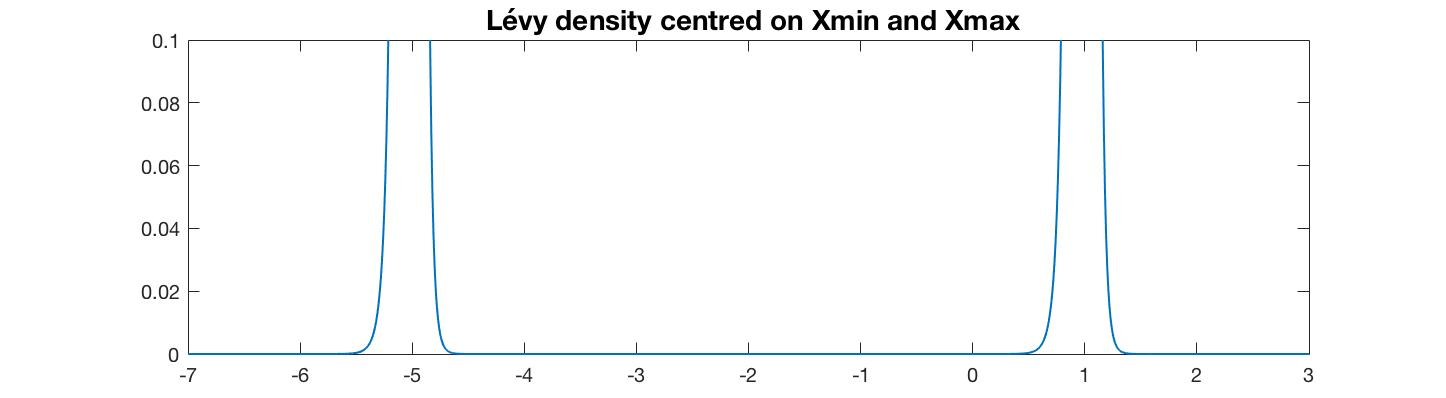
\includegraphics[width=\textwidth]{gfx/qmin_qmax}
	\caption{L\'evy density centered on $x_{\min}$ and $x_{\max}$ to justify the choice of $q_{\min}$ and $q_{\max}$.}
	\label{fig:qmin-qmax}
\end{figure}

For the Convolution method, we took the same values for $x_{\min}$ and $x_{\max}$ than the Finite Difference method.

Finally, the grids discretization per scenario is summarized in table \ref{tab:settings}. 

\begin{table}[!ht]
\centering
  \begin{tabular}{l||c|c|c}
    \toprule
    Scenarios & Monte Carlo & Finite Difference & Convolution \\
    \toprule
   	I 	& $M=10^2$ & $N_x=250,N_a=25,N_t=5$    & $N_x=250,N_a=25$\\
  	II 	& $M=10^3$ & $N_x=500,N_a=50,N_t=10$   & $N_x=500,N_a=50$\\
    III & $M=10^4$ & $N_x=1000,N_a=100,N_t=20$ & $N_x=1000,N_a=100$\\
    IV 	& $M=10^5$ & $N_x=2000,N_a=200,N_t=40$ & $N_x=2000,N_a=200$\\
    V 	& $M=10^6$ & $N_x=4000,N_a=400,N_t=80$ & $N_x=4000,N_a=400$\\
    \bottomrule
  \end{tabular}
  \vspace{5pt}
  \caption{\label{tab:settings} Number of simulations per Monte Carlo scenario and grids discretization for the FD and Conv methods.}
\end{table}

\subsection{Results tables}
All the numerical results are listed in Tables \ref{tab:res_ng} to \ref{tab:res_fg} at the end of the chapter.

\section{Speed, Accuracy and Convergence analysis}
\label{sec:res:analysis}
This section is devoted to the analysis of the results. We will first briefly discuss the Monte Carlo method before study the performances of the Finite Difference method and Convolution method.

\subsection{Monte Carlo method analysis}
First of all, let's see the decay of the standard error with respect to the number of simulation $M$ illustrated in Figure \ref{fig:MC_error}. As expected, the error decays with the ratio $1/\sqrt{M}$. This method gives good results from $M = 10^6$ but it is very expensive in computational time, especially for the jump diffusion models where we have to simulate jumps independently of the Brownian path. In this case, we can see in the results tables that the CPU time explode for the Merton and Kou model. Therefore, it is not a good choice to use Monte Carlo method for pricing options when other numerical methods are available.

\begin{figure}[!htb]
\centering
	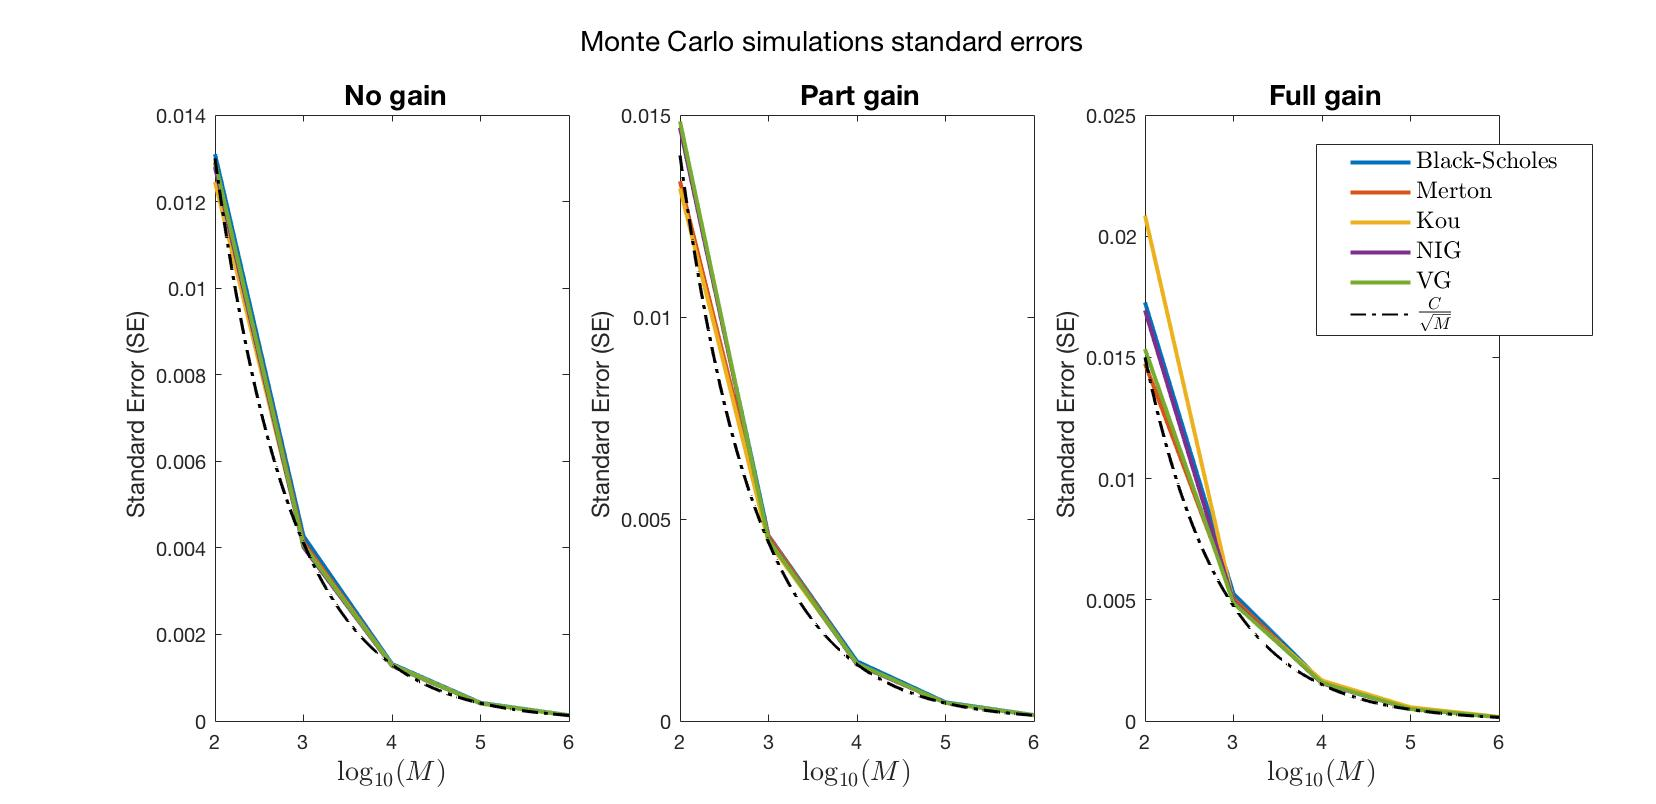
\includegraphics[width=\textwidth]{gfx/MC_error}
	\caption{Monte Carlo standard error analysis.}
	\label{fig:MC_error}
\end{figure}

\subsection{Convergence analysis}
Let's now check the convergence of the Finite Difference method and the Convolution method. In Figure \ref{fig:fd_conv} and \ref{fig:conv_conv}, we plot the convergence error of the two methods. 

\begin{figure}[!htb]
\centering
	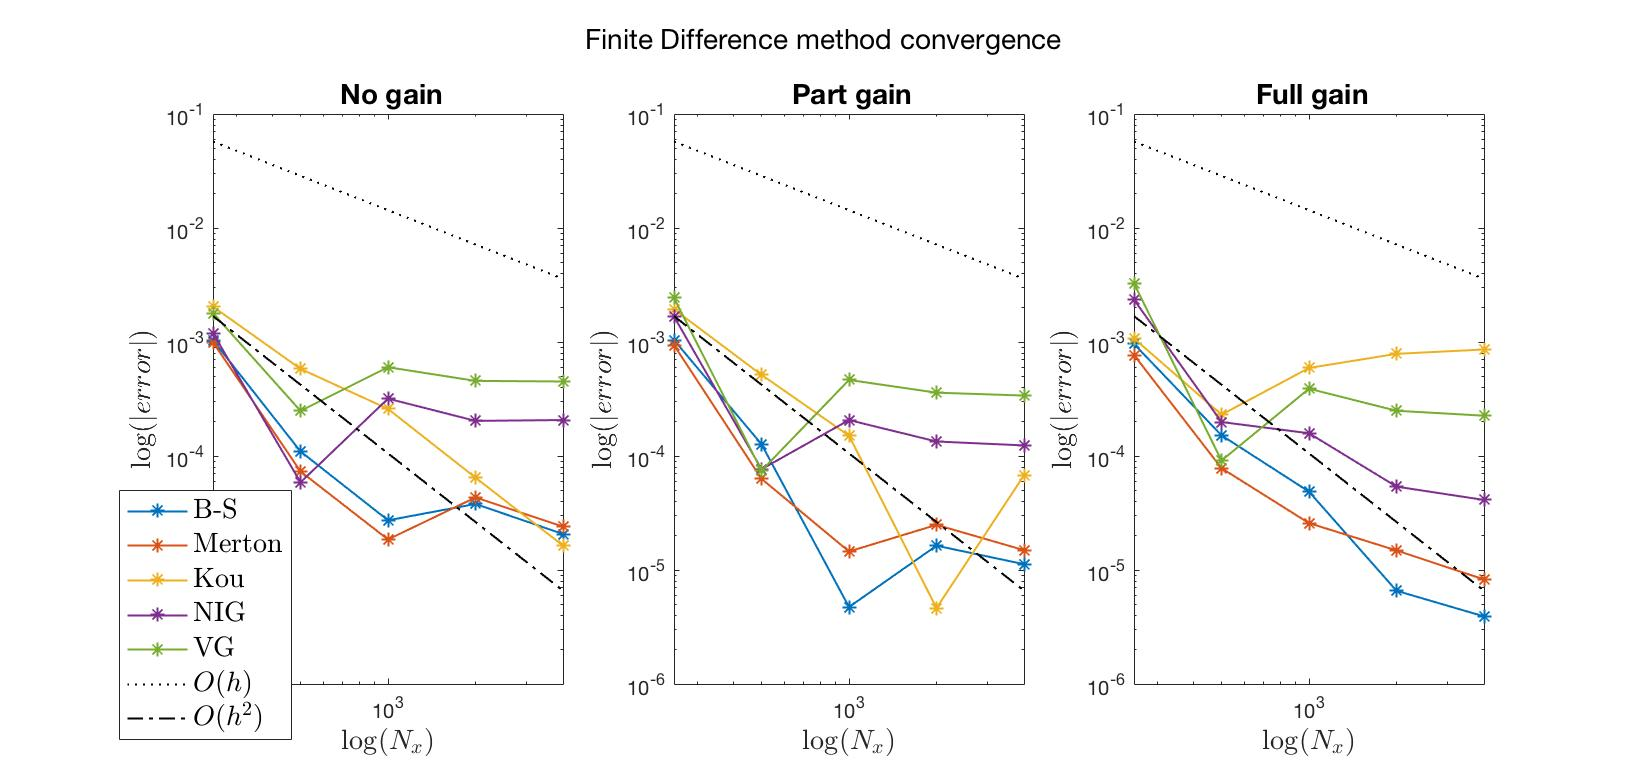
\includegraphics[width=\textwidth]{gfx/FD_convergence}
	\caption{Convergence of the Finite Difference method.}
	\label{fig:fd_conv}
\end{figure}

\begin{figure}[!htb]
\centering
	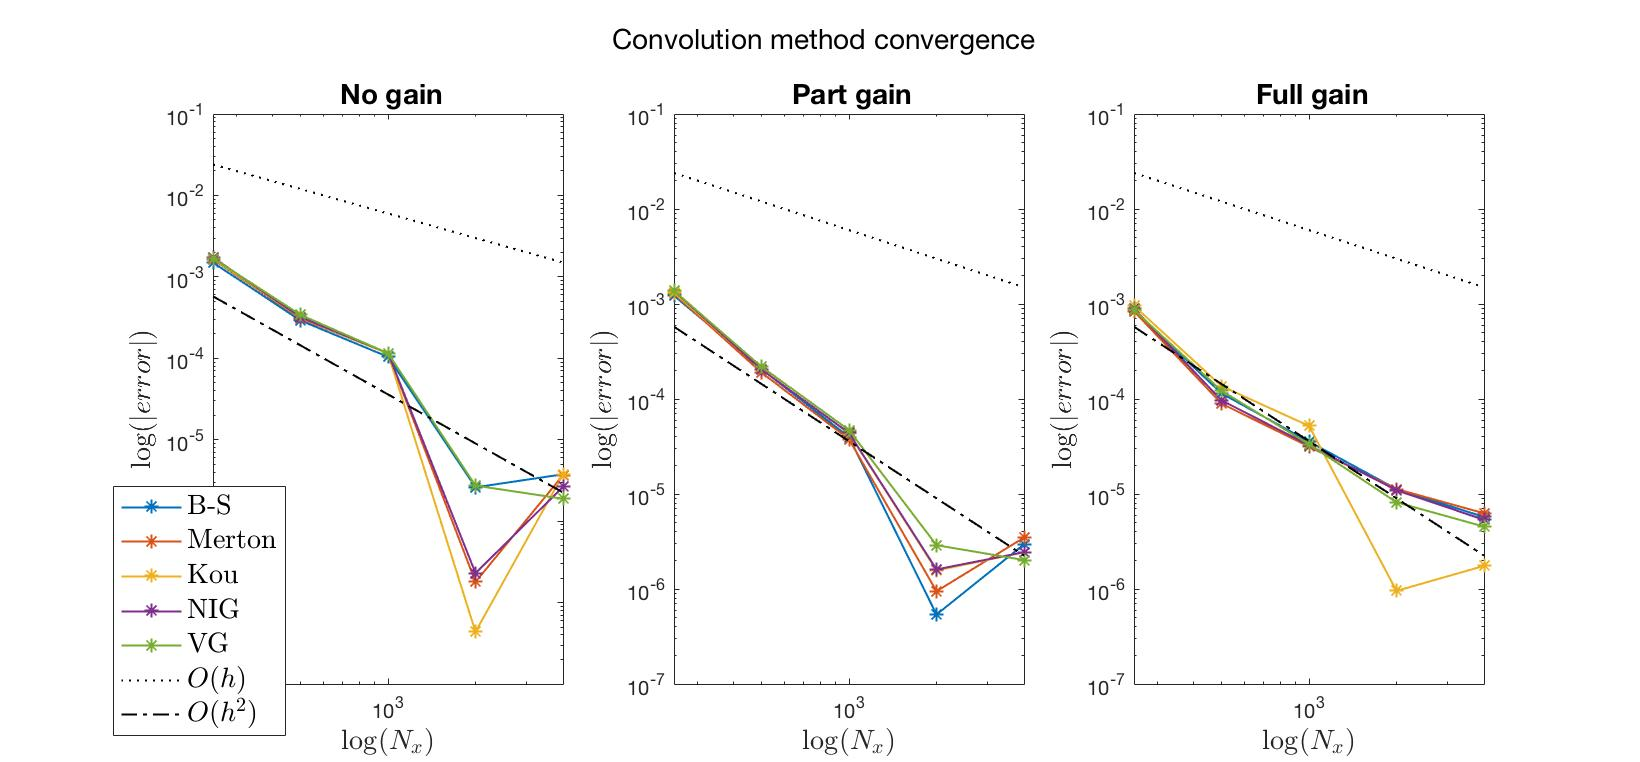
\includegraphics[width=\textwidth]{gfx/Conv_convergence}
	\caption{Convergence of the Convolution method.}
	\label{fig:conv_conv}
\end{figure}

We can see that the Convolution method has a convergence order 2 while the Finite Difference method has difficulties to converge for pure jump models. This is certainly due to the truncation in the L\'evy density. Therefore, the method converges to this truncation error. Here, since the Convolution method uses the characteristic function in its closed form without modification or approximation, we have fewer losses in the accuracy.

\subsection{Speed and accuracy analysis}
It can be interesting to compare the speed and accuracy of these both numerical methods to make a good choice for pricing engine. At the top of the Figure \ref{fig:speed}, we can see the accuracy of the methods with respect to the computational time. And at the bottom, the running time in function of the grid points number $N_x$.

\begin{figure}[!htb]
\centering
	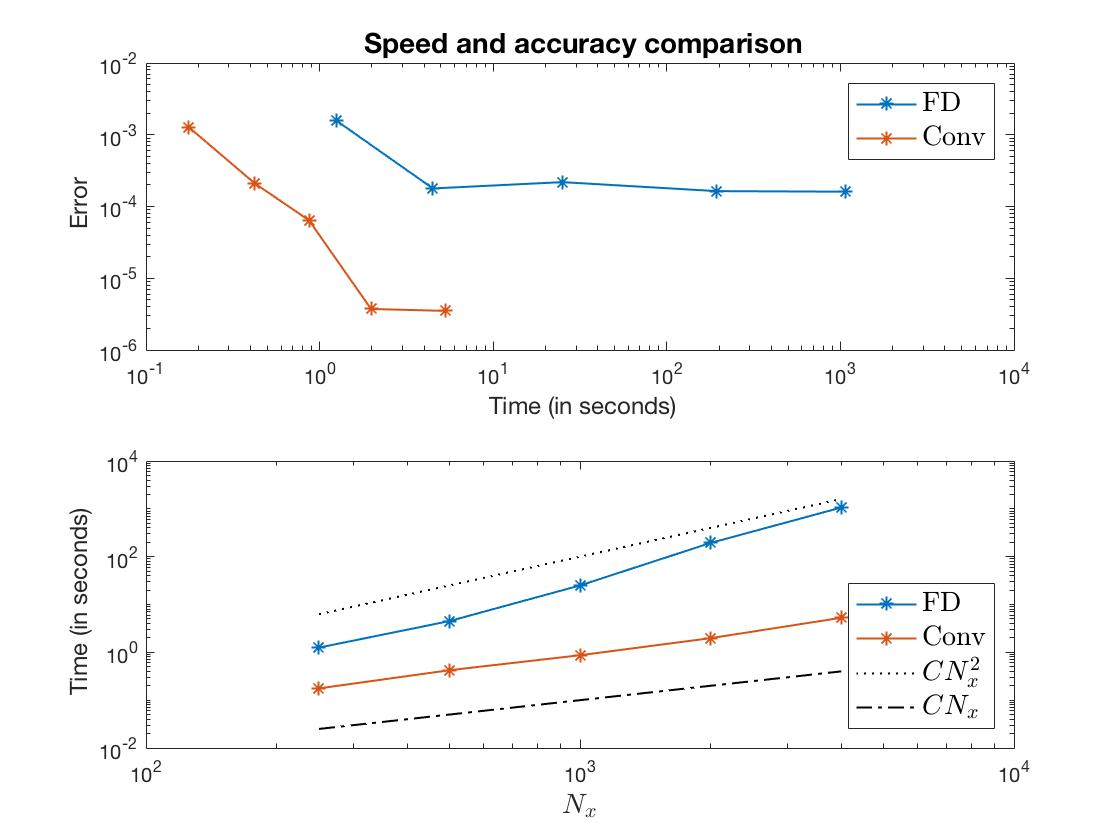
\includegraphics[width=\textwidth]{gfx/speed}
	\caption{Speed and accuracy comparison between the FD method and the Conv method. At the top: Error in function of computational time. At the bottom: Running time in function of $N_x$.}
	\label{fig:speed}
\end{figure}

In addition to being much faster than Finite Difference method, the Convolution method is more precise. In fact, he Convolution method grows up linearly with respect to the number of grid points $N_x$, while the Finite Difference method grows up quadratically. Finally, for the same accuracy, the Convolution method can be from 13 to 15 times faster than the Finite Difference method.

The gain in accuracy from $N_x = 2000$ to $N_x = 4000$ in the Convolution method is not very important. Thus it seems to be a good compromise to choose the Convolution method with $N_x = 2000$ to price our FX-TARN option.

\section{Value of the term sheet example}
\label{sec:res:TS}
We arrive to the goal of the project that is to price a real case of FX-TARN. We will then compute three different prices which are
\begin{itemize}
\item A bid price, obtained from the calibration on the bid volatility quotes,
\item A mid price, obtained from the calibration on the mid volatility quotes,
\item An ask price, obtained from the calibration on the ask volatility quotes.
\end{itemize}

We use, as discussed before, the Convolution method, with $N_x = 2000$ and $N_a = 200$, to price the FX-TARN of the term sheet example. The prices are given in Table \ref{tab:prices}.

\begin{table}[!ht]
\centering
  \begin{tabular}{l||c|c|c||c}
    \toprule
    \textbf{FX-TARN} & Bid & Mid & Ask & RMSE \\
    \toprule
   Black-Scholes 	& CHF $-21'204$ & CHF $-23'197$ & CHF $-25'202$ & 10.2e-04\\
   Merton 			& CHF $-17'713$ & CHF $-19'960$ & CHF $-22'104$ & 3.05e-04\\
   Kou 				& CHF $-18'348$ & CHF $-21'193$ & CHF $-23'812$ & 2.79e-04\\
   NIG 				& CHF $-17'409$ & CHF $-19'252$ & CHF $-20'983$ & 4.97e-04\\
   VG 				& CHF $-17'692$ & CHF $-19'506$ & CHF $-21'160$ & 5.88e-04\\
    \bottomrule
  \end{tabular}
  \vspace{5pt}
  \caption{\label{tab:prices} Prices of the FX-TARN for all the models. The RMSE is the mean of the three RMSE per model. Each price is computed in 19 seconds.}
\end{table}

The negative value means that the client will receive a premium when signing the contract. The price given by a trader to the client will depend on his book and the risk premium he would like to take. The most representative price with respect to the market is the prices given by the Kou model because its RMSE is the smallest. Then, a fair premium for the client would be around CHF 18'300.-, where the risk is include in the volatility price. Then, the risk premium of the trader would be around CHF 5'500.-, which is the difference with the ask price.

\begin{sidewaystable}[!ht]
\centering
  \begin{tabular}{l||c|c|c||c|c|c||c|c|c}
    \toprule
    \textbf{No Gain} & \multicolumn{3}{c||}{\textbf{Monte Carlo}} & \multicolumn{3}{c||}{\textbf{Finite Difference}} & \multicolumn{3}{c}{\textbf{Convolution}} \\
    \toprule
    Black-Scholes ($V_\text{ref}= 0.15877$) & Value & Std Error  & Time & Value & Error & Time & Value & Error & Time \\
      \midrule
    Scenario I   & 0.14932 & 1.31e-02 & 0.01 & 0.15774 & 1.03e-03 & 1.11 & 0.15728 & 1.50e-03 & 0.19 \\
    Scenario II  & 0.15863 & 4.27e-03 & 0.02 & 0.15866 & 1.10e-04 & 4.94 & 0.15848 & 2.91e-04 & 0.36 \\
    Scenario III & 0.15676 & 1.32e-03 & 0.10 & 0.15875 & 2.73e-05 & 28.8 & 0.15867 & 1.04e-04 & 0.80 \\
    Scenario IV  & 0.15870 & 4.20e-04 & 0.50 & 0.15881 & 3.80e-05 & 192  & 0.15878 & 2.60e-06 & 1.71 \\
    Scenario V   & 0.15859 & 1.33e-04 & 4.77 & 0.15879 & 2.07e-05 & 1244 & 0.15878 & 3.76e-06 & 4.85 \\
     \midrule
      Merton ($V_\text{ref}=0.15929$) & Value & Std Error  & Time & Value & Error & Time & Value & Error & Time \\
      \midrule
    Scenario I   & 0.16950 & 1.29e-02 & 0.06 & 0.15829 & 9.94e-04 & 0.98 & 0.15765 & 1.64e-03 & 0.16\\
    Scenario II  & 0.16485 & 4.13e-03 & 0.28 & 0.15921 & 7.32e-05 & 4.64 & 0.15898 & 3.08e-04 & 0.34\\
    Scenario III & 0.15834 & 1.29e-03 & 1.89 & 0.15927 & 1.85e-05 & 27.3 & 0.15917 & 1.14e-08 & 0.79\\
    Scenario IV  & 0.15968 & 4.07e-04 & 16.3 & 0.15933 & 4.33e-05 & 187  & 0.15929 & 1.79e-07 & 1.87\\
    Scenario V   & 0.15920 & 1.29e-04 & 184  & 0.15931 & 2.40e-05 & 1094 & 0.15929 & 3.67e-06 & 5.59\\
     \midrule
      Kou ($V_\text{ref}=0.15792$) & Value & Std Error  & Time & Value & Error & Time & Value & Error & Time \\
      \midrule
    Scenario I   & 0.14190 & 1.24e-02 & 0.11 & 0.15588 & 2.04e-03 & 0.94 & 0.15624 & 1.68e-03 & 0.18 \\
    Scenario II  & 0.15042 & 4.06e-03 & 0.77 & 0.15733 & 5.81e-04 & 4.42 & 0.15760 & 3.14e-04 & 0.35 \\
    Scenario III & 0.15837 & 1.30e-03 & 6.05 & 0.15766 & 2.59e-04 & 22.1 & 0.15780 & 1.14e-04 & 0.75 \\
    Scenario IV  & 0.15823 & 4.08e-04 & 60.2 & 0.15785 & 6.46e-05 & 183  & 0.15792 & 4.37e-08 & 1.83 \\
    Scenario V   & 0.15789 & 1.29e-04 & 689  & 0.15790 & 1.64e-05 & 1077 & 0.15792 & 3.74e-06 & 6.25 \\
         \midrule
      NIG ($V_\text{ref}=0.16166$) & Value & Std Error  & Time & Value & Error & Time & Value & Error & Time \\
      \midrule
    Scenario I   & 0.13656 & 1.28e-02 & 0.02 & 0.16285 & 1.19e-03 & 1.25 & 0.15992 & 1.73e-03 & 0.16\\
    Scenario II  & 0.15641 & 4.01e-03 & 0.04 & 0.16160 & 5.88e-05 & 5.00 & 0.16134 & 3.19e-04 & 0.40\\
    Scenario III & 0.16377 & 1.27e-03 & 0.11 & 0.16134 & 3.19e-04 & 22.2 & 0.16154 & 1.16e-04 & 0.74\\
    Scenario IV  & 0.16166 & 4.04e-04 & 0.60 & 0.16145 & 2.03e-04 & 184  & 0.16166 & 2.30e-07 & 1.80\\
    Scenario V   & 0.16179 & 1.28e-04 & 6.29 & 0.16145 & 2.07e-04 & 1078 & 0.16166 & 2.63e-06 & 5.87\\
         \midrule
      VG ($V_\text{ref}=0.16246$) & Value & Std Error  & Time & Value & Error & Time & Value & Error & Time \\
      \midrule
    Scenario I   & 0.16907 & 1.29e-03 & 0.01 & 0.16426 & 1.79e-03 & 1.26 & 0.16077 & 1.69e-03 & 0.15\\
    Scenario II  & 0.15588 & 4.05e-04 & 0.02 & 0.16222 & 2.49e-04 & 5.43 & 0.16212 & 3.41e-04 & 0.33\\
    Scenario III & 0.16314 & 1.28e-04 & 0.18 & 0.16186 & 6.01e-04 & 22.3 & 0.16235 & 1.15e-04 & 0.77\\
    Scenario IV  & 0.16235 & 4.06e-04 & 0.61 & 0.16201 & 4.56e-04 & 184  & 0.16246 & 2.73e-06 & 1.86\\
    Scenario V   & 0.16227 & 1.29e-04 & 6.04 & 0.16201 & 4.50e-04 & 1050 & 0.16247 & 1.88e-06 & 5.21\\
    \bottomrule
  \end{tabular}
  \vspace{5pt}
  \caption{\label{tab:res_ng} Results of No Gain TARN. The error in FD and Conv methods are given by $|V(S_0,t_0,0)-V_\text{ref}(V(S_0,t_0,0)|$ and the CPU Times are expressed in seconds.}
\end{sidewaystable}

\begin{sidewaystable}[!ht]
\centering
  \begin{tabular}{l||c|c|c||c|c|c||c|c|c}
    \toprule
    \textbf{Part Gain} & \multicolumn{3}{c||}{\textbf{Monte Carlo}} & \multicolumn{3}{c||}{\textbf{Finite Difference}} & \multicolumn{3}{c}{\textbf{Convolution}} \\
    \toprule
    Black-Scholes ($V_\text{ref}= 0.16863$) & Value & Std Error  & Time & Value & Error & Time & Value & Error & Time \\
      \midrule
    Scenario I   & 0.16856 & 1.47e-02 & 0.01 & 0.16759 & 1.04e-03 & 1.14 & 0.16740 & 1.22e-03 & 0.17\\
    Scenario II  & 0.16711 & 4.59e-03 & 0.03 & 0.16850 & 1.27e-04 & 5.18 & 0.16842 & 2.06e-04 & 0.32\\
    Scenario III & 0.17228 & 1.48e-03 & 0.11 & 0.16862 & 4.73e-05 & 23.0 & 0.16859 & 3.97e-05 & 0.74\\
    Scenario IV  & 0.16863 & 4.62e-04 & 0.53 & 0.16864 & 1.63e-05 & 200  & 0.16863 & 5.39e-07 & 2.11\\
    Scenario V   & 0.16841 & 1.46e-04 & 5.05 & 0.16864 & 1.12e-05 & 1197 & 0.16863 & 2.95e-06 & 4.85\\
     \midrule
      Merton ($V_\text{ref}=0.16854$) & Value & Std Error  & Time & Value & Error & Time & Value & Error & Time \\
      \midrule
    Scenario I   & 0.18279 & 1.34e-02 & 0.05 & 0.16760 & 9.40e-04 & 0.95 & 0.16726 & 1.28e-03 & 0.14 \\
    Scenario II  & 0.17194 & 4.57e-03 & 0.20 & 0.16848 & 6.31e-05 & 3.88 & 0.16835 & 1.90e-04 & 0.35 \\
    Scenario III & 0.16990 & 1.41e-03 & 1.72 & 0.16856 & 1.45e-05 & 23.7 & 0.16850 & 3.77e-05 & 0.94 \\
    Scenario IV  & 0.16865 & 4.48e-04 & 18.2 & 0.16857 & 2.49e-05 & 194  & 0.16854 & 9.47e-07 & 2.06 \\
    Scenario V   & 0.16870 & 1.42e-04 & 164  & 0.16856 & 1.49e-05 & 1019 & 0.16854 & 3.48e-06 & 5.34 \\
     \midrule
      Kou ($V_\text{ref}=0.16688$) & Value & Std Error  & Time & Value & Error & Time & Value & Error & Time \\
      \midrule
    Scenario I   & 0.16444 & 1.32e-02 & 0.09 & 0.16495 & 1.93e-03 & 1.19 & 0.16557 & 1.31e-03 & 0.18 \\
    Scenario II  & 0.16616 & 4.43e-03 & 0.67 & 0.16637 & 5.15e-04 & 4.07 & 0.16668 & 2.05e-04 & 0.40 \\
    Scenario III & 0.16508 & 1.42e-03 & 6.97 & 0.16673 & 1.51e-04 & 24.2 & 0.16684 & 4.35e-05 & 0.82 \\
    Scenario IV  & 0.16675 & 4.46e-04 & 70.5 & 0.16689 & 4.63e-06 & 198  & 0.16688 & 1.57e-06 & 2.14\\
    Scenario V   & 0.16676 & 1.41e-04 & 604  & 0.16695 & 6.77e-05 & 992  & 0.16688 & 2.43e-06 & 5.12\\
         \midrule
      NIG ($V_\text{ref}=0.17093$) & Value & Std Error  & Time & Value & Error & Time & Value & Error & Time \\
      \midrule
    Scenario I   & 0.20942 & 1.47e-02 & 0.01 & 0.17261 & 1.67e-03 & 1.43 & 0.16956 & 1.37e-03 & 0.18 \\
    Scenario II  & 0.17137 & 4.50e-03 & 0.04 & 0.17101 & 7.66e-05 & 4.23 & 0.17073 & 2.04e-04 & 0.45 \\
    Scenario III & 0.17025 & 1.40e-03 & 0.10 & 0.17072 & 2.07e-04 & 24.7 & 0.17089 & 4.39e-05 & 0.86 \\
    Scenario IV  & 0.17054 & 4.45e-04 & 0.67 & 0.17080 & 1.34e-04 & 196  & 0.17093 & 1.61e-06 & 2.18 \\
    Scenario V   & 0.17094 & 1.41e-04 & 5.43 & 0.17081 & 1.24e-04 & 1064 & 0.17093 & 2.44e-06 & 5.73 \\
         \midrule
      VG ($V_\text{ref}=0.17181$) & Value & Std Error  & Time & Value & Error & Time & Value & Error & Time \\
      \midrule
    Scenario I   & 0.18370 & 1.48e-02 & 0.01 & 0.17424 & 2.43e-03 & 1.97 & 0.17043 & 1.38e-03 & 0.22\\
    Scenario II  & 0.17527 & 4.48e-03 & 0.01 & 0.17173 & 7.43e-05 & 4.43 & 0.17159 & 2.18e-04 & 0.35\\
    Scenario III & 0.17162 & 1.42e-03 & 0.09 & 0.17134 & 4.65e-04 & 24.2 & 0.17176 & 4.71e-05 & 0.90\\
    Scenario IV  & 0.17091 & 4.47e-04 & 0.67 & 0.17145 & 3.59e-04 & 200  & 0.17181 & 2.89e-06 & 2.29\\
    Scenario V   & 0.17182 & 1.42e-04 & 6.40 & 0.17147 & 3.39e-04 & 1086 & 0.17181 & 2.01e-06 & 5.30\\
    \bottomrule
  \end{tabular}
  \vspace{5pt}
  \caption{\label{tab:res_pg} Results of Part Gain TARN. The error in FD and Conv methods are given by $|V(S_0,t_0,0)-V_\text{ref}(V(S_0,t_0,0)|$ and the CPU Times are expressed in seconds.}
\end{sidewaystable}

\begin{sidewaystable}[!ht]
\centering
  \begin{tabular}{l||c|c|c||c|c|c||c|c|c}
    \toprule
    \textbf{Full Gain} & \multicolumn{3}{c||}{\textbf{Monte Carlo}} & \multicolumn{3}{c||}{\textbf{Finite Difference}} & \multicolumn{3}{c}{\textbf{Convolution}} \\
    \toprule
    Black-Scholes ($V_\text{ref}= 0.17763$) & Value & Std Error  & Time & Value & Error & Time & Value & Error & Time \\
      \midrule
    Scenario I   & 0.17144 & 1.73e-02 & 0.01 & 0.17667 & 9.61e-04 & 1.31 & 0.17678 & 8.23e-01 & 0.19\\
    Scenario II  & 0.17773 & 5.25e-03 & 0.02 & 0.17748 & 1.52e-04 & 4.89 & 0.17751 & 1.15e-04 & 0.31 \\
    Scenario III & 0.17749 & 1.62e-03 & 0.07 & 0.17758 & 4.87e-05 & 26.9 & 0.17759 & 3.56e-05 & 0.71 \\
    Scenario IV  & 0.17670 & 5.13e-04 & 0.54 & 0.17763 & 6.57e-06 & 193 & 0.17764 & 1.13e-05 & 1.75 \\
    Scenario V   & 0.17756 & 1.62e-04 & 4.50 & 0.17763 & 3.92e-06 & 1116 & 0.17763 & 5.73e-06 & 4.59 \\
     \midrule
      Merton ($V_\text{ref}=0.17687$) & Value & Std Error  & Time & Value & Error & Time & Value & Error & Time \\
      \midrule
    Scenario I   & 0.16647 & 1.47e-02 & 0.03 & 0.17610 & 7.69e-04 & 1.10 & 0.17603 & 8.39e-04 & 0.17 \\
    Scenario II  & 0.18610 & 5.05e-03 & 0.21 & 0.17679 & 7.82e-05 & 4.02 & 0.17678 & 8.95e-05 & 0.33 \\
    Scenario III & 0.17616 & 1.58e-03 & 2.08 & 0.17684 & 2.58e-05 & 26.3 & 0.17683 & 3.15e-05 & 1.26 \\
    Scenario IV  & 0.17605 & 4.97e-04 & 16.5 & 0.17688 & 1.48e-05 & 199 & 0.17688 & 1.13e-05 & 1.91 \\
    Scenario V   & 0.17701 & 1.58e-04 & 161  & 0.17687 & 8.27e-05 & 989 & 0.17687 & 6.26e-06 & 5.24 \\
     \midrule
      Kou ($V_\text{ref}=0.17534$) & Value & Std Error  & Time & Value & Error & Time & Value & Error & Time \\
      \midrule
    Scenario I   & 0.21626 & 2.09e-02 & 0.10 & 0.17427 & 1.07e-03 & 1.09 & 0.17439 & 9.56e-04 & 0.19 \\
    Scenario II  & 0.17653 & 4.86e-03 & 0.64 & 0.17557 & 2.30e-04 & 4.01 & 0.17521 & 1.37e-04 & 0.35 \\
    Scenario III & 0.17956 & 1.67e-03 & 7.64 & 0.17593 & 5.92e-04 & 27.0 & 0.17529 & 5.21e-05 & 1.25 \\
    Scenario IV  & 0.17655 & 5.67e-04 & 68.4 & 0.17613 & 7.87e-04 & 196 & 0.17534 & 9.55e-07 & 2.27 \\
    Scenario V   & 0.17645 & 1.69e-04 & 589  & 0.17620 & 8.59e-04 & 989 & 0.17534 & 1.75e-06 & 4.96 \\
         \midrule
      NIG ($V_\text{ref}=0.17929$) & Value & Std Error  & Time & Value & Error & Time & Value & Error & Time \\
      \midrule
    Scenario I   & 0.20382 & 1.69e-02 & 0.01 & 0.18164 & 2.35e-03 & 1.54 & 0.17840 & 8.93e-04 & 0.20 \\
    Scenario II  & 0.17687 & 4.91e-03 & 0.03 & 0.17949 & 1.99e-04 & 4.07 & 0.17920 & 9.68e-05 & 0.35 \\
    Scenario III & 0.17872 & 1.55e-03 & 0.11 & 0.17913 & 1.58e-04 & 26.9 & 0.17926 & 3.27e-05 & 0.81 \\
    Scenario IV  & 0.17910 & 4.95e-04 & 0.61 & 0.17924 & 5.39e-05 & 203 & 0.17930 & 1.09e-05 & 2.06 \\
    Scenario V   & 0.17923 & 1.57e-04 & 6.38 & 0.17925 & 4.12e-05 & 989 & 0.17930 & 5.35e-06 & 5.20 \\
         \midrule
      VG ($V_\text{ref}=0.18024$) & Value & Std Error  & Time & Value & Error & Time & Value & Error & Time \\
      \midrule
    Scenario I   & 0.18783 & 1.53e-02 & 0.01 & 0.18350 & 3.26e-03 & 1.53 & 0.17937 & 8.65e-04 & 0.16 \\
    Scenario II  & 0.17395 & 4.86e-03 & 0.03 & 0.18033 & 9.11e-05 & 4.21 & 0.18011 & 1.22e-04 & 0.35 \\
    Scenario III & 0.18189 & 1.58e-03 & 0.11 & 0.17985 & 3.89e-04 & 25.5 & 0.18020 & 3.34e-05 & 0.89 \\
    Scenario IV  & 0.17998 & 4.97e-04 & 0.66 & 0.17999 & 2.49e-04 & 201 & 0.18024 & 8.18e-06 & 1.84 \\
    Scenario V   & 0.18017 & 1.57e-04 & 5.60 & 0.18001 & 2.26e-04 & 990 & 0.18024 & 4.54e-06 & 5.11 \\
    \bottomrule
  \end{tabular}
  \vspace{5pt}
  \caption{\label{tab:res_fg} Results of Full Gain TARN. The error in FD and Conv methods are given by $|V(S_0,t_0,0)-V_\text{ref}(V(S_0,t_0,0)|$ and the CPU Times are expressed in seconds.}
\end{sidewaystable}

